\documentclass[10pt,a4paper]{article}
\usepackage{tocloft}
\usepackage{commons/course}  % همین کافیه؛ listings و xcolor داخلشه
\usepackage{booktabs}

% Define colors for syntax highlighting
\definecolor{keywordstyle}{rgb}{0.0, 0.4, 0.8} % A bluer shade
\definecolor{stringstyle}{rgb}{0.9, 0.17, 0.31} % amaranth
\definecolor{commentstyle}{rgb}{0.1, 0.6, 0.2} % green
\definecolor{numberstyle}{rgb}{0.4, 0.4, 0.4} % gray
\definecolor{backgroundcolor}{rgb}{0.94, 0.97, 1.0} % aliceblue

% Define the Python-like language for syntax highlighting
\lstdefinelanguage{PythonLike}{
	morekeywords={mov, add, sub, cmp, jmp , lw , addi,sw,bne},
	sensitive=false,
	morecomment=[l]{;},
	morestring=[b]",
}

% Set the style for Python-like code
\lstset{
	language=PythonLike,
	basicstyle=\ttfamily\small,
	keywordstyle=\color{keywordstyle},
	stringstyle=\color{stringstyle},
	commentstyle=\color{commentstyle},
	numbers=left,
	numberstyle=\tiny\color{numberstyle},
	stepnumber=1,
	numbersep=5pt,
	keepspaces=true,
	tabsize=4,
	showspaces=false,
	showstringspaces=false,
	showtabs=false,
	breaklines=true,
	breakatwhitespace=false,
	frame=single,
	backgroundcolor=\color{backgroundcolor},
}

\newlistof{listofproblems}{lop}{\normalsize فهرست مسائل}
\newcommand{\addproblem}[1]{\addcontentsline{lop}{listofproblems}{\protect\numberline{}#1}}


\begin{document}


\سربرگ{آزمایش چهارم}{جمع‌کننده/تفریق‌کننده ممیز شناور}{معین آعلی - ثمین اکبری}{استاد: دکتر حمید سربازی آزاد}

\subsubsection*{خلاصه}

در این آزمایش یک جمع‌کننده/تفریق‌کننده‌ی ممیز شناور ۳۲ بیتی مطابق استاندارد \lr{IEEE754} در نرم‌افزار \lr{Logisim} طراحی و پیاده‌سازی شده است. مدار به‌صورت تک‌سطحی و ترکیبی از قطعات آماده‌ی کتابخانه‌ی \lr{Arithmetic} و \lr{Plexers} ساخته شده: \lr{Comparator} برای مقایسه‌ی نماها، \lr{Shifter} برای هم‌ترازسازی و نرمال‌سازی مانتیس، \lr{Adder}/\lr{Subtractor} برای ترکیب مانتیس‌ها، و \lr{Priority Encoder} برای یافتن موقعیت اولین بیت ۱ در مرحله‌ی نرمال‌سازی.



\subsubsection*{دیاگرام کلی مدار}
\begin{figure}[h]
  \centering
  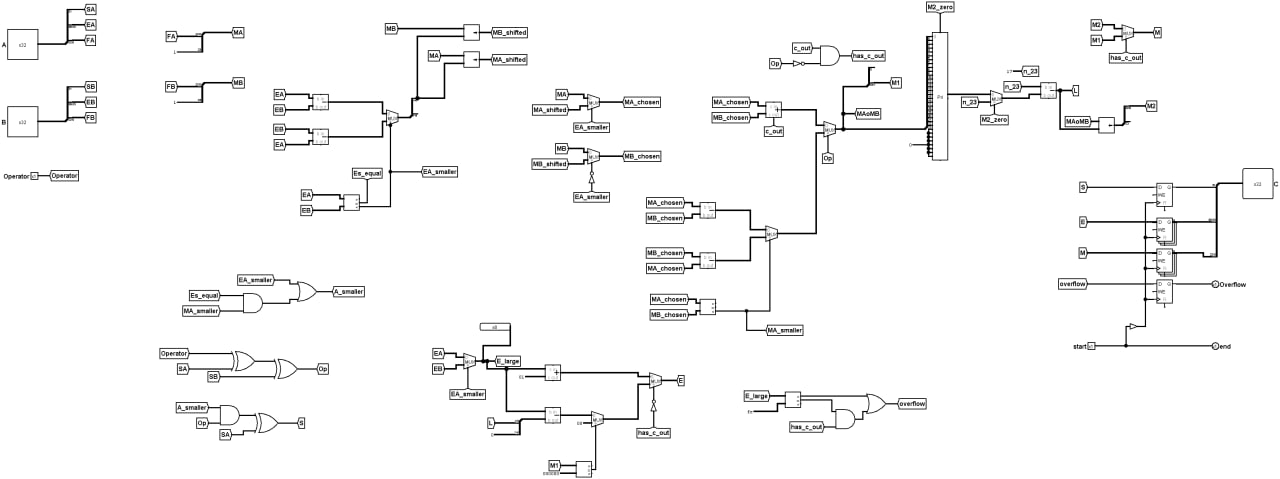
\includegraphics[width=0.95\textwidth]{figs/full.jpg}
\end{figure}


\subsubsection*{هدف آزمایش}

هدف از این آزمایش، آشنایی عملی با قالب نمایش \lr{IEEE754} و پیاده‌سازی یک واحد جمع/تفریق ممیز شناور ۳۲ بیتی است. برخلاف جمع صحیح، جمع دو عدد ممیز شناور به مراحل هم‌ترازسازی نما، جمع/تفریق مانتیس، و نرمال‌سازی نتیجه نیاز دارد. اهداف مشخص این آزمایش عبارت‌اند از:

\begin{itemize}
  \item آشنایی عملی با قالب نمایش \lr{IEEE754} و نحوه‌ی رمزگشایی/رمزگذاری آن با علامت، نما و مانتیس.
  \item پیاده‌سازی مرحله‌ی هم‌ترازسازی نما (\lr{Alignment}) پیش از جمع دو عدد ممیز شناور.
  \item پیاده‌سازی جمع/تفریق مانتیس با در نظر گرفتن علامت عملوندها و رقم نقلی.
  \item پیاده‌سازی مرحله‌ی نرمال‌سازی نتیجه و تشخیص سرریز نما.
\end{itemize}


\subsubsection*{قالب \lr{IEEE754}}

هر عدد ۳۲ بیتی به‌صورت زیر رمزگذاری می‌شود:
\[
\text{Value} = (-1)^{S} \times 1.M \times 2^{E-127}
\]

\begin{center}
\begin{tabular}{@{}llll@{}}
\toprule
\textbf{فیلد} & \textbf{بیت‌ها} & \textbf{پهنا} & \textbf{توضیح} \\
\midrule
\lr{S} (علامت) & ۳۱ & ۱ & ۰ مثبت، ۱ منفی \\
\lr{E} (نما) & ۳۰..۲۳ & ۸ & نمای بایاس‌شده با بایاس ۱۲۷ \\
\lr{M} (مانتیس) & ۲۲..۰ & ۲۳ & قسمت کسری؛ بیت پنهان \lr{1.} صریح ذخیره نمی‌شود \\
\bottomrule
\end{tabular}
\end{center}


\subsubsection*{رابط مدار}

\begin{center}
\begin{tabular}{@{}llll@{}}
\toprule
\textbf{سیگنال} & \textbf{جهت} & \textbf{پهنا} & \textbf{توضیح} \\
\midrule
\lr{A}, \lr{B} & ورودی & ۳۲ & عملوندها، قالب \lr{IEEE754} \\
\lr{Operator} & ورودی & ۱ & \lr{0} جمع ($A+B$)، \lr{1} تفریق ($A-B$) \\
\lr{C} & خروجی & ۳۲ & حاصل جمع یا تفریق، قالب \lr{IEEE754} \\
\lr{Overflow} & خروجی & ۱ & سرریز نما (قفل‌شده) \\
\lr{start} & ورودی & ۱ & با لبه‌ی بالارونده، محاسبه‌ی جاری را روی خروجی قفل می‌کند \\
\lr{end} & خروجی & ۱ & هم‌زمان با \lr{start} فعال است؛ اعتبار خروجی را نشان می‌دهد \\
\bottomrule
\end{tabular}
\end{center}

مدار در پنج مرحله کار می‌کند که در ادامه توضیح داده می‌شوند.


\subsubsection*{مرحله ۱ — استخراج فیلدها و هم‌ترازسازی نما}

با یک \lr{Splitter} روی هرکدام از \lr{A} و \lr{B}، فیلدهای \lr{S}، \lr{E} و \lr{M} جدا می‌شوند و بیت پنهان \lr{1} به ابتدای مانتیس اضافه می‌شود تا یک عدد ۲۴ بیتی $1.M$ ساخته شود (\lr{MA} و \lr{MB}).

نماها با یک \lr{Comparator} (حالت \lr{unsigned}) مقایسه می‌شوند تا $E_{\mathrm{large}} = \max(E_A, E_B)$ مشخص شود. اختلاف نماها با یک \lr{Subtractor} محاسبه و مانتیس عملوند کوچک‌تر با یک \lr{Shifter} (شیفت منطقی راست) به همان اندازه شیفت داده می‌شود تا هر دو مانتیس روی مقیاس $E_{\mathrm{large}}$ هم‌تراز شوند:
\[
M_{\mathrm{small,aligned}} = M_{\mathrm{small}} \gg (E_{\mathrm{large}} - E_{\mathrm{small}})
\]

{
\centering{
  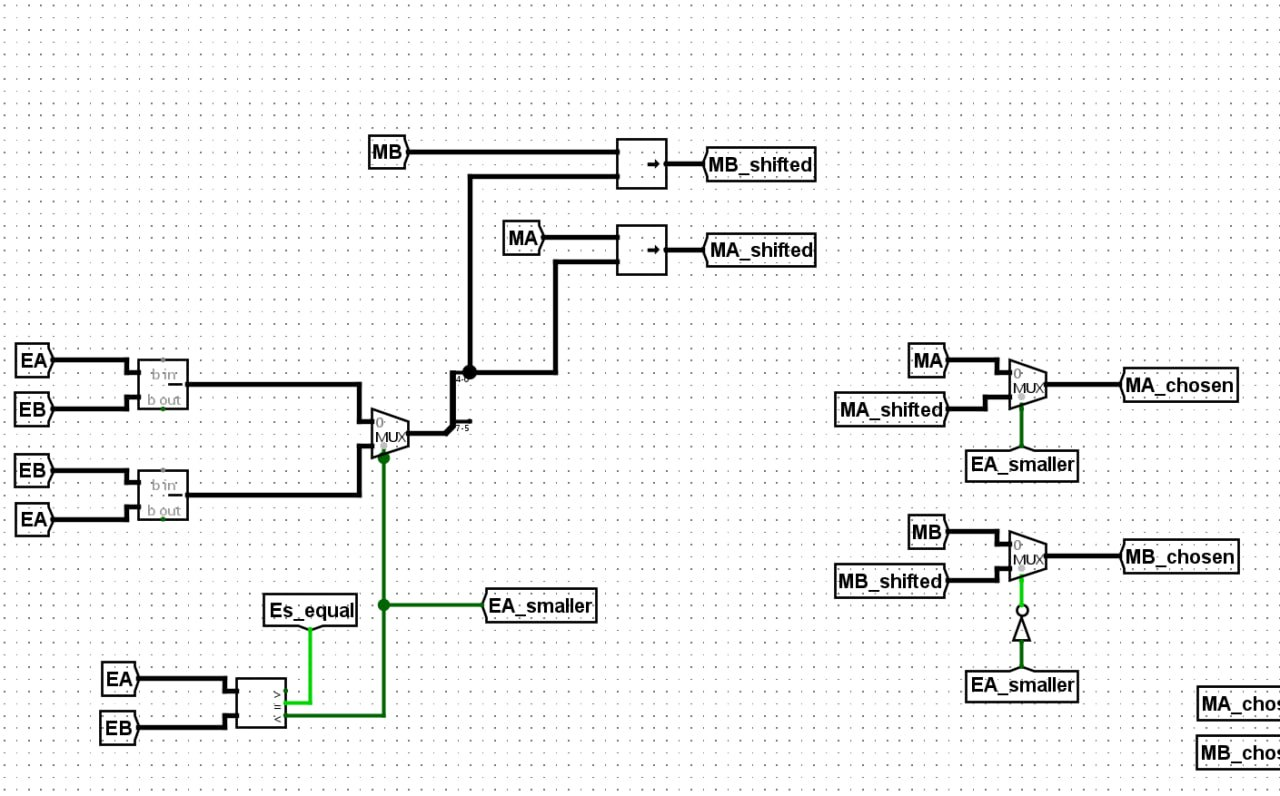
\includegraphics[width=0.95\textwidth]{figs/align.jpg}
}
}


\subsubsection*{مرحله ۲ — تعیین عملیات مؤثر و علامت}

چون جمع دو عدد با علامت مخالف معادل تفریق است (و برعکس)، عملیات مؤثر روی مانتیس‌ها با \lr{XOR} کردن \lr{Operator} و علامت عملوندها به دست می‌آید:
\[
\mathrm{Op} = \mathrm{Operator} \oplus S_B
\]

هم‌زمان اندازه‌ی دو عملوند به‌طور کامل (نه فقط نما) با ترکیب خروجی \lr{Comparator} نماها و یک \lr{Comparator} روی مانتیس‌ها مقایسه می‌شود:
\[
A_{\mathrm{smaller}} = (E_A < E_B) \lor \big((E_A = E_B) \land (M_A < M_B)\big)
\]

علامت نتیجه از عملوند بزرگ‌تر گرفته می‌شود؛ در حالت $\mathrm{Op}=1$ (تفریق مؤثر) اگر عملوند کوچک‌تر انتخاب‌شونده تغییر کند، علامت نیز معکوس می‌شود.


\subsubsection*{مرحله ۳ — جمع/تفریق مانتیس}

بسته به $\mathrm{Op}$، مانتیس‌های هم‌ترازشده وارد یک \lr{Adder} ۲۴ بیتی یا یک \lr{Subtractor} ۲۴ بیتی می‌شوند (تفریق همیشه به‌صورت بزرگ‌تر منهای کوچک‌تر انجام می‌شود، پس هرگز رقم قرضی ایجاد نمی‌کند). در حالت جمع، بیت رقم نقلی خروجی (\lr{has\_c\_out}) نشان می‌دهد نتیجه از ۲۳ بیت (یعنی از بازه‌ی \lr{1.xxx}) فراتر رفته و باید یک بیت به راست شیفت داده و نمای خروجی یک واحد افزایش یابد. در این حالت یک رقم ۱ داریم و نیازی به شیفت بیشتر عدد برای نرمال‌سازی نیست.


\subsubsection*{مرحله ۴ — نرمال‌سازی و تشخیص سرریز}

اگر جمع رقم نقلی تولید نکرده باشد (یا عملیات تفریق بوده)، ممکن است بیت پیشرو (\lr{1}) در موقعیتی پایین‌تر از بیت ۲۳ افتاده باشد. یک \lr{Priority Encoder} موقعیت اولین بیت ۱ مانتیس ۲۴ بیتی را پیدا می‌کند؛ تعداد شیفت لازم برای نرمال‌سازی از تفاضل این موقعیت با ۲۳ به دست می‌آید و مانتیس با یک \lr{Shifter} نهایی به همان اندازه به چپ شیفت داده می‌شود. نمای خروجی هم به همان اندازه کاهش می‌یابد (یا در حالت رقم نقلی، یک واحد افزایش می‌یابد).

سرریز نما با مقایسه‌ی نمای نهایی (\lr{unsigned}) با مقدار \lr{0xFE} (۲۵۴) تشخیص داده می‌شود — بزرگ‌ترین نمای مجاز پیش از رزروشدن کد \lr{0xFF}:
\[
\mathrm{Overflow} = (E_{\mathrm{final}} > 254) \lor \big((E_{\mathrm{final}} = 254) \land c_{\mathrm{out}}\big)
\]

{
\centering{
  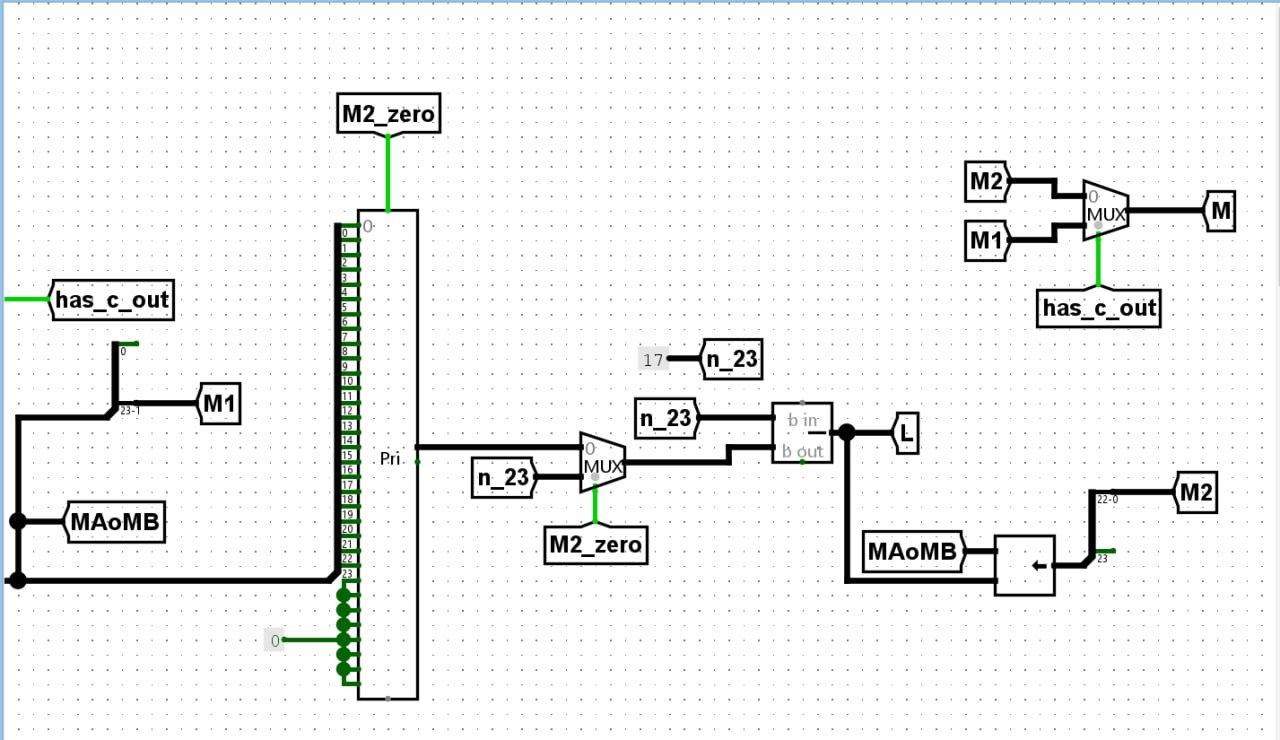
\includegraphics[width=0.95\textwidth]{figs/normal1.jpg}
}
}

{
\centering{
  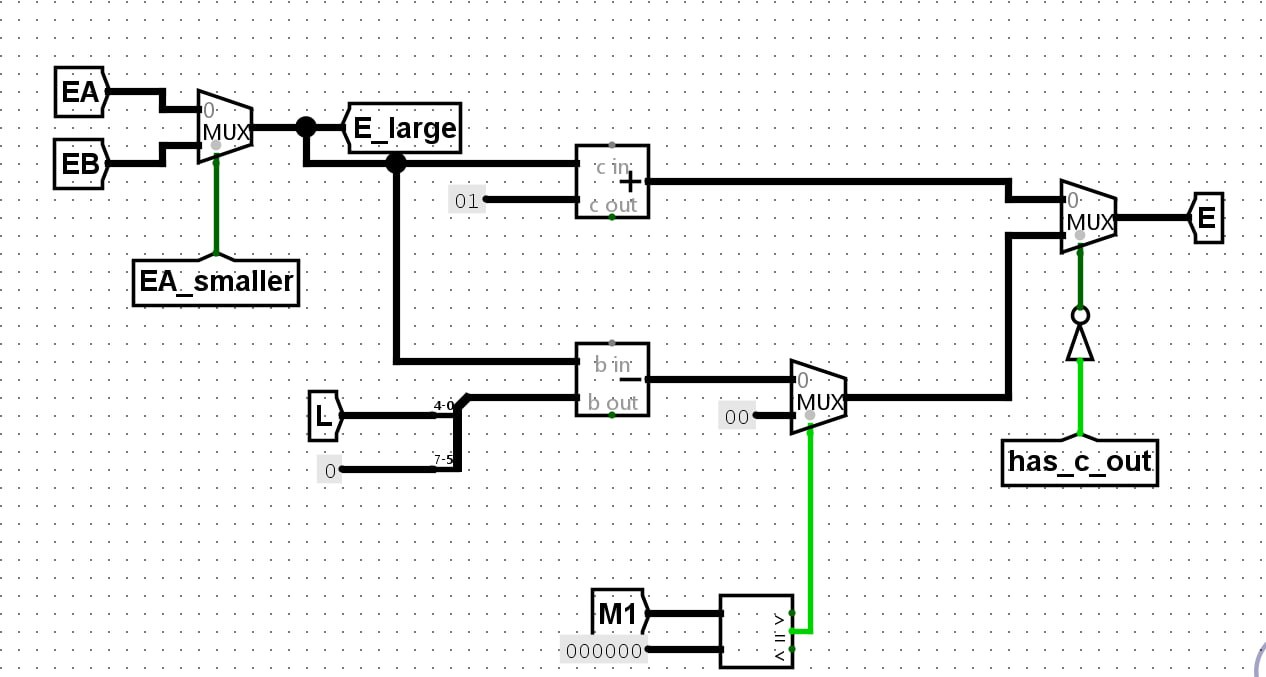
\includegraphics[width=0.95\textwidth]{figs/normal2.jpg}
}
}


\pagebreak


\subsubsection*{مرحله ۵ — واحد قفل خروجی (\lr{start}/\lr{end})}

بخش‌های ۱ تا ۴ کاملاً ترکیبی‌اند و همیشه در حال محاسبه‌ی مقدار جدید بر اساس \lr{A}، \lr{B} و \lr{Operator} جاری هستند. برای اینکه خروجی فقط با فرمان صریح به‌روز شود، هرکدام از چهار فیلد نتیجه (\lr{Sign}، \lr{Exponent}، \lr{Mantissa}، \lr{Overflow}) از یک \lr{Register} عبور می‌کند پیش از رسیدن به پایه‌ی خروجی:
\[
Q \leftarrow D \quad \text{در لبه‌ی بالارونده‌ی } clk
\]

هر چهار رجیستر با یک کلاک مشترک، از \lr{start} ساخته می‌شوند. تا وقتی $\mathrm{start}=0$ است، رجیسترها آخرین مقدار قفل‌شده را نگه می‌دارند؛ با لبه‌ی بالارونده‌ی \lr{start}، مقدار لحظه‌ای محاسبه‌شده ثبت و روی خروجی ظاهر می‌شود. سیگنال \lr{end} مستقیماً از همان پایه‌ی \lr{start} گرفته می‌شود (از طریق یک گیت \lr{Buffer} که آن را از کلاک جدا نگه می‌دارد) و هم‌زمان با \lr{start} فعال است — چون منطق محاسبه ترکیبی است، به‌محض عبور لبه‌ی کلاک مقدار جدید در دسترس است و نیازی به تأخیر یا شمارش سیکل نیست.

{
\centering{
  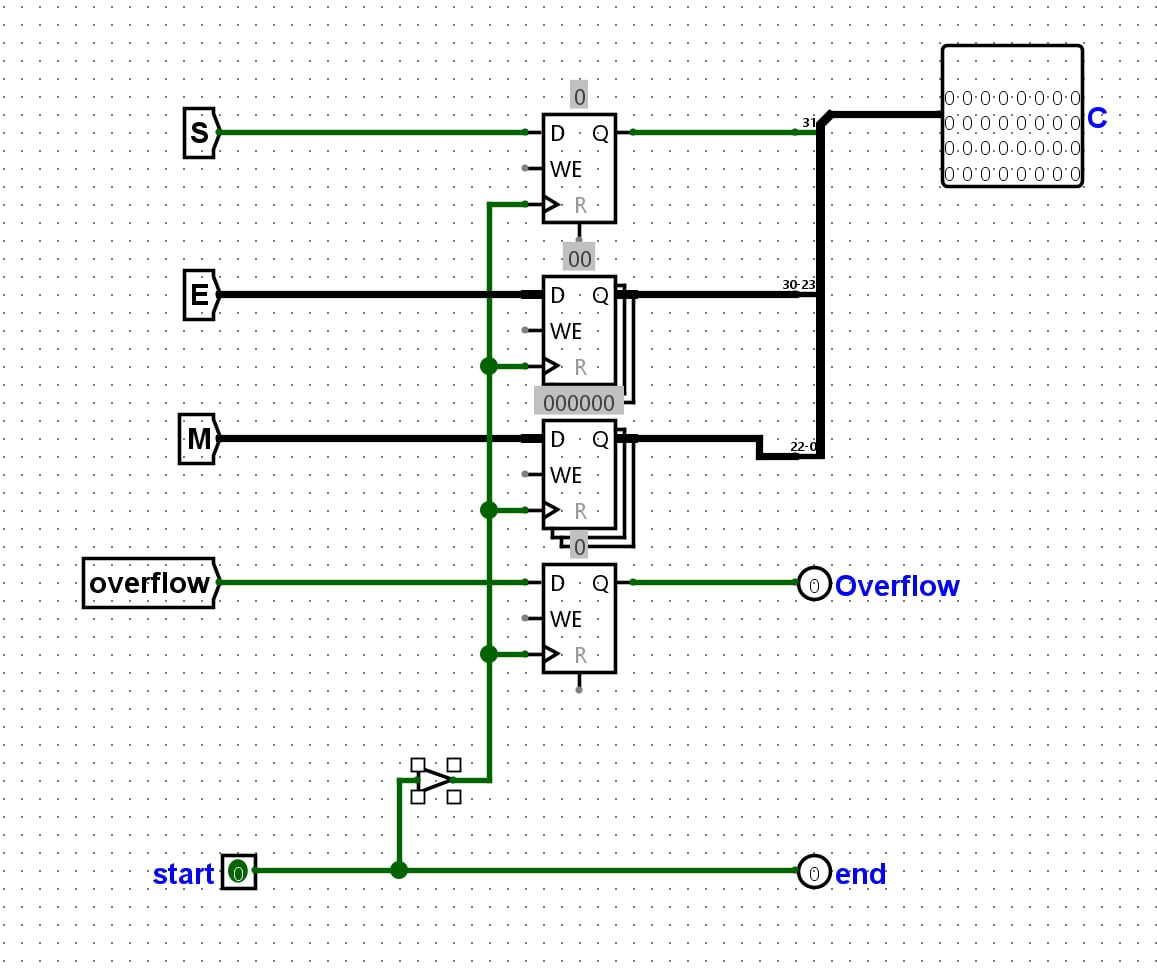
\includegraphics[width=0.95\textwidth]{figs/output.jpg}
}
}



\end{document}
